\documentclass[a4paper,12pt]{article} % добавить leqno в [] для нумерации слева
\usepackage[a4paper,top=1.3cm,bottom=2cm,left=1.5cm,right=1.5cm,marginparwidth=0.75cm]{geometry}
%%% Работа с русским языком
\usepackage{cmap}					% поиск в PDF
\usepackage{mathtext} 				% русские буквы в фомулах
\usepackage[T2A]{fontenc}			% кодировка
\usepackage[utf8]{inputenc}			% кодировка исходного текста
\usepackage[english,russian]{babel}	% локализация и переносы
\usepackage{multirow}

\usepackage{graphicx}

\usepackage{wrapfig}
\usepackage{tabularx}

\usepackage{hyperref}
\usepackage[rgb]{xcolor}
\hypersetup{
colorlinks=true,urlcolor=blue
}

%%% Дополнительная работа с математикой
\usepackage{amsmath,amsfonts,amssymb,amsthm,mathtools} % AMS
\usepackage{icomma} % "Умная" запятая: $0,2$ --- число, $0, 2$ --- перечисление

%% Номера формул
\mathtoolsset{showonlyrefs=true} % Показывать номера только у тех формул, на которые есть \eqref{} в тексте.

%% Шрифты
\usepackage{euscript}	 % Шрифт Евклид
\usepackage{mathrsfs} % Красивый матшрифт

%% Свои команды
\DeclareMathOperator{\sgn}{\mathop{sgn}}

%% Перенос знаков в формулах (по Львовскому)
\newcommand*{\hm}[1]{#1\nobreak\discretionary{}
{\hbox{$\mathsurround=0pt #1$}}{}}

%% Графики
\usepackage{tikz}
\usepackage{pgfplots}
\pgfplotsset{compat=1.9}

\date{\today}

\begin{document}

\begin{titlepage}
	\begin{center}
		{\large МОСКОВСКИЙ ФИЗИКО-ТЕХНИЧЕСКИЙ ИНСТИТУТ (НАЦИОНАЛЬНЫЙ ИССЛЕДОВАТЕЛЬСКИЙ УНИВЕРСИТЕТ)}
	\end{center}
	\begin{center}
		{\large Физтех-школа аэрокосмических технологий}
	\end{center}
	
	
	\vspace{4.5cm}
	{\huge
		\begin{center}
			{\bf Отчёт о выполнении лабораторной работы 2.1.3}\\
			Определение $C_P/C_V$ по скорости звука в газе
		\end{center}
	}
	\vspace{1cm}
	\begin{center}
		{\large Соболевский Федор Александрович \\
			\vspace{0.2cm}
			Б03-109}
	\end{center}
	\vspace{8cm}
	\begin{center}
		Апрель 2022
	\end{center}
\end{titlepage}

\section{Аннотация}

В данной работе с помощью определения резонансных частот найдена скорость звука в различных газах. По скорости звука из уравнения идеального газа определён показатель адиабаты газов. Вычислены и проанализированы систематические и случайные погрешности, оценена применимость модели идеального газа для вычисления скорости звука.

\section{Теоретические сведения}

\subsection{Скорость звука в газе}

Скорость звука в идеальном газе определяется формулой

\begin{equation}
    c = \sqrt{\gamma\frac{RT}{\mu}},
\end{equation}

где $R$ - универсальная газовая постоянная, $T$ - температура газа, $\mu$ - его молярная масса, $\gamma$ - его показатель адиабаты. Преобразуя данную формулу, получаем выражение для показателя адиабаты

\begin{equation}
    \gamma = \frac{\mu}{RT}c^2.
    \label{gamma}
\end{equation}

При распространении звука в газе в трубе резонанс - резкое увеличение амплитуды колебаний - возникает, когда в длину трубы укладывается целое число полуволн, то есть

\begin{equation}
    L = n\frac{\lambda}{2}, \text{    } n \in \mathbb{N}.
\end{equation}

Здесь $L$ - длина трубы, $\lambda$ - длина звуковой волны. Скорость звуковой волны связана с её длиной и частотой $f$ соотношением 

\begin{equation}
    c = \lambda f.
    \label{sonic}
\end{equation}

Подбор условий возникновения резонанса можно производить двумя способами:

1. При неизменной частоте звукогенератора менять длину трубы. Для последовательных резонансов при неизменной длине волны имеем:

\begin{equation}
    L_n = n\frac{\lambda}{2} \text{,        } L_{n + k} = n\frac{\lambda}{2} + k\frac{\lambda}{2}.
    \label{cor1}
\end{equation}

В этом случае величина $\lambda/2$ равна коэффициенту наклона графика зависимости длины трубы от номера резонанса.

2. При постоянной длине трубы изменять частоты звукогенератора. Для последовательных резонансов имеем

\begin{equation}
    L = \frac{\lambda_1}{2}n = \frac{\lambda_2}{2}(n + 1) = \dots = \frac{\lambda_{k+1}}{2}(n + k).
    \label{freaqs}
\end{equation}

Из \eqref{sonic} и \eqref{freaqs} имеем

\begin{equation*}
    \begin{array}{ccc}
    \centering
        f_1 = \frac{c}{\lambda_1} = \frac{c}{2L}n, & f_2 = \frac{c}{\lambda_2} = \frac{c}{2L}(n + 1) = f_1 + \frac{c}{2L}, & \dots ,\\ \\
        & f_{k + 1} = \frac{c}{\lambda_{k+1}} = f_1 + \frac{c}{2L}k.
    \end{array}
\end{equation*}

Скорость звука определяется из углового коэффициента наклона графика зависимости резонансной частоты от номера резонанса.

\subsection{Экспериментальная установка}

\begin{figure}
    \centering
    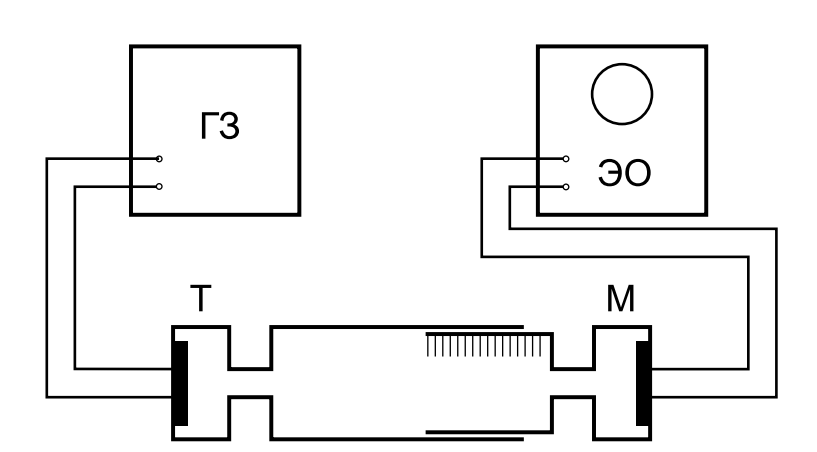
\includegraphics[width = 0.65\textwidth]{setup1.PNG}
    \caption{Установка для измерения скорости звука при помощи раздвижной трубы}
    \label{fig:setup1}
\end{figure}

\begin{figure}
    \centering
    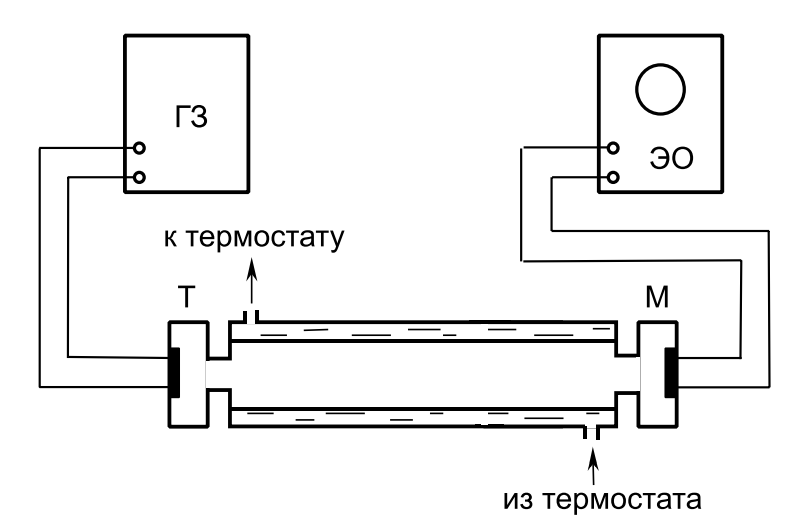
\includegraphics[width = 0.65\textwidth]{setup2.PNG}
    \caption{Установка для изучения зависимости скорости звука от температуры}
    \label{fig:setup2}
\end{figure}

Соответственно двум методам измерения скорости звука в работе были использованы две установки (рис. \ref{fig:setup1} и \ref{fig:setup2}). В обеих установках звуковые колебания в трубе возбуждались телефоном Т и улавливались микрофоном М. Мембрана телефона приводима в движение переменным током звуковой частоты; в качестве источника переменной ЭДС использовался звуковой генератор ГЗ. Возникающий в микрофоне сигнал наблюдался на осциллографе ЭО.

Микрофон и телефон присоединены к установке через тонкие резиновые трубки. Такая связь достаточна для возбуждения и обнаружения звуковых колебаний в трубе и в то же время мало возмущает эти колебания: при расчетах оба торца трубы можно считать неподвижными, а влиянием соединительных отверстий пренебречь.

Первая установка (рис. \ref{fig:setup1}) содержит раздвижную трубу с миллиметровой шкалой. Через патрубок (на рисунке не показан) труба может наполняться воздухом или углекислым газом из газгольдера. На этой установке производились измерения показателя адиабаты для воздуха и для CO$_2$. Вторая установка (рис. \ref{fig:setup2}) содержит теплоизолированную трубу постоянной длины. Воздух в трубе нагревался водой из термостата. Температура газа принимается равной температуре омывающей трубу воды. На этой установке измерялась зависимость скорости звука от температуры.

\section{Оборудование и инструментальные погрешности}

\textbf{В работе использовались:} звуковой генератор ГЗ; электронный
осциллограф ЭО; микрофон; телефон; частотометр; раздвижная труба с линейкой; теплоизолированная труба, обогреваемая водой из термостата; баллон со сжатым углекислым газом; газгольдер.

\textbf{Инструментальные погрешности:} 

\begin{itemize}
    \item \textbf{Линейка:} $\Delta_L = 1$ мм;
    \item \textbf{Частотометр:} $\Delta_f = 1$ Гц; 
    \item \textbf{Термометр термостата:} $\Delta_T = 0,1$ К.
\end{itemize}

\section{Результаты измерений и обработка экспериментальных данных}

\subsection{Измерение скорости звука на первой установке}

Измерения на первой установке проводились для воздуха и для углекислого газа. Начальная длина раздвижной трубы $L_0 = 570 \pm 1$ мм, комнатная температура - 24,8 $^\text{o}$C. 

Для набора частот были найдены соответствующие резонансу длины трубы. По этим данным были построены зависимости резонансных длин от их номера. Графики данных зависимостей изображены на рис. \ref{graph:air} и \ref{graph:CO2}. Далее методом наименьших квадратов были найдены угловые коэффициенты наилучших прямых, равные из \eqref{cor1} $\lambda/2$. Отсюда по формуле \eqref{sonic} была найдена скорость звука для каждого измерения. Результаты измерений представлены в таблице \ref{tab:exp1}.

По результатам опыта с углекислым газом видно, что полученные значения скорости звука гораздо ближе к табличному значению для воздуха ($c_\text{air} = 334$ м/с), чем для углекислого газа ($c_\text{CO$_2$} = 260$ м/с). Это говорит о том, что при проведении измерений для углекислого газа в установку натекло значительное количество воздуха, из-за чего результаты эксперимента ошибочны. Из-за этого в дальнейшем будут рассматриваться только значения скорости звука в воздухе.

\begin{figure}
\centering
\resizebox {0.55\textwidth} {!} {
\begin{tikzpicture}
\begin{axis}[ xlabel = {$k$}, ylabel = {$\Delta L_k$}, xmin = 0, xmax = 7, ymin = 0, ymax = 22, legend style={legend style={at={(axis cs:7, 0)},anchor=south east}}]
\addplot[color=black, mark=star, only marks] coordinates{
(1, 5.4)
(2, 15.6)};
\addplot[color=black, mark=o, only marks] coordinates{
(1, 4.2)
(2, 10.9)
(3, 17.6)};
\addplot[color=black, mark=*, only marks] coordinates{
(1, 3.3)
(2, 8.4)
(3, 13.3)
(4, 18.4)};
\addplot[color=black, mark=square, only marks] coordinates{
(1, 4.7)
(2, 8.8)
(3, 12.9)
(4, 16.9)
(5, 21)};
\addplot[color=black, mark=triangle, only marks] coordinates{
(1, 1.4)
(2, 4.7)
(3, 8.1)
(4, 11.5)
(5, 14.8)
(6, 18.2)};
\legend{$f_1$, $f_2$, $f_3$, $f_4$, $f_5$}
\addplot[color=blue] coordinates{(1, 5.4)(2, 15.6)};
\addplot[color=red] coordinates{(1, 4.2)(3, 17.6)};
\addplot[color=purple] coordinates{(1, 3.3)(4, 18.3)};
\addplot[color=blue] coordinates{(1, 4.2)(5, 21)};
\addplot[color=red] coordinates{(1, 1.4)(6, 18.15)};
\end{axis}
\end{tikzpicture}
}
\caption{Резонансные длины трубы для воздуха}
\label{graph:air}
\end{figure}

\begin{figure}
\centering
\resizebox {0.55\textwidth} {!} {
\begin{tikzpicture}
\begin{axis}[ xlabel = {$k$}, ylabel = {$\Delta L_k$}, xmin = 0, xmax = 7, ymin = 0, ymax = 22, legend style={legend style={at={(axis cs:7, 0)},anchor=south east}}]
\addplot[color=black, mark=star, only marks] coordinates{
(1, 1.4)
(2, 15.6)};
\addplot[color=black, mark=o, only marks] coordinates{
(1, 4.4)
(2, 13.1)
(3, 21.8)};
\addplot[color=black, mark=*, only marks] coordinates{
(1, 0.1)
(2, 6.3)
(3, 12.7)
(4, 18.9)};
\addplot[color=black, mark=square, only marks] coordinates{
(1, 2.1)
(2, 7.0)
(3, 11.8)
(4, 16.7)
(5, 21.6)};
\addplot[color=black, mark=triangle, only marks] coordinates{
(1, 0.8)
(2, 5)
(3, 9)
(4, 13.1)
(5, 17.2)
(6, 21.2)};
\legend{$f_1$, $f_2$, $f_3$, $f_4$, $f_5$}
\addplot[color=blue] coordinates{(1, 1.4)(2, 15.6)};
\addplot[color=red] coordinates{(1, 4.4)(3, 21.8)};
\addplot[color=purple] coordinates{(1, 0.1)(4, 18.95)};
\addplot[color=blue] coordinates{(1, 2.1)(5, 21.6)};
\addplot[color=red] coordinates{(1, 0.8)(6, 21.3)};
\end{axis}
\end{tikzpicture}
}
\caption{Резонансные длины трубы для углекислого газа}
\label{graph:CO2}
\end{figure}

\begin{table}[]
    \centering
    \begin{tabular}{|c|c|c|c|c|}\hline
        \multicolumn{5}{|c|}{Воздух} \\ \hline
        $f$, кГц & $\Delta L_\text{рез}$, см & $k = \lambda/2$, см & $\lambda$, м & $c$, м/с \\ \hline
        1,7 & 5,4; 15,6 & 10,2 & 0,204 & 346,8 \\ \hline
        2,55 & 4,2; 10,9; 17,6 & 6,7 & 0,134 & 341,7 \\ \hline
        3,4 & 3,3; 8,4; 13,3; 18,4 & 5,0 & 0,100 & 341,4 \\ \hline
        4,25 & 4,7; 8,8; 12,9; 16,9; 21,0 & 4,1 & 0,081 & 346,0 \\ \hline
        5,1 & 1,4; 4,7; 8,1; 11,5; 14,8; 18,2 & 3,4 & 0,067 & 343,0 \\ \hline
        \multicolumn{5}{|c|}{Углекислый газ} \\ \hline
        $f$, кГц & $\Delta L_\text{рез}$, см & $k = \lambda/2$, см & $\lambda$, м & $c$, м/с \\ \hline
        1,1 & 1,4; 15,6 & 14,2 & 0,284 & 312,4 \\ \hline
        1,6 & 4,4; 13,1; 21,8 & 8,7 & 0,174 & 278,4 \\ \hline
        2,7 & 0,1; 6,3; 12,7; 18,9 & 6,3 & 0,126 & 339,1 \\ \hline
        3,5 & 2,1; 7,0; 11,8; 16,7; 21,6 & 4,9 & 0,097 & 340,9 \\ \hline
        4,2 & 0,8; 5,0; 9,0; 13,1; 17,2; 21,2 & 4,1 & 0,082 & 342,5 \\ \hline
    \end{tabular}
    \caption{Результаты вычисления скорости звука с помощью раздвижной трубы}
    \label{tab:exp1}
\end{table}

По результатам опыта можно определить среднее значение скорости звука, случайную, систематическую и полную погрешность его определения:

\begin{equation*}
\begin{array}{c}
    \overline{c} = \frac{1}{5}\sum c_i = 343,8 \text{ м/с}, \\
     \\
    \sigma_c^\text{случ} = \sqrt{\frac{1}{5 \cdot 4}\sum (c_i - \overline{c})^2} = 1,1 \text{ м/с}, \\
     \\
    \sigma_c^\text{сист} = c\sqrt{(\frac{\Delta_f}{f})^2 + (\frac{2\Delta_L}{\lambda})^2} = 6,9 \text{ м/с}, \\ 
     \\
    \sigma_c^\text{полн} = \sqrt{(\sigma_c^\text{сист})^2 + (\sigma_c^\text{случ})^2} = 7 \text{ м/с}.
\end{array}
\end{equation*}

Итоговое значение скорости звука в воздухе в первом опыте:

\begin{itemize}
    \item $c_1 = 344 \pm 7$ м/с. 
\end{itemize}

Отсюда можно найти по формуле \eqref{gamma} показатель адиабаты и определить погрешность его измерения:

\begin{equation*}
\begin{array}{c}
    \gamma = \frac{\mu}{RT}c^2 = 1,38 \\
     \\
    \sigma_\gamma = \gamma\sqrt{(\frac{\Delta_T}{T})^2 + 2^2(\frac{\sigma_c^\text{полн}}{c})^2} = 0,06 
\end{array}
\end{equation*}

Итоговое значение показателя адиабаты воздуха в первом опыте:

\begin{itemize}
    \item $\gamma = 1,38 \pm 0,06$. 
\end{itemize}

\subsection{Измерение скорости звука на второй установке}

Во втором опыте измерения проводились на установке с трубой постоянной длины $L = 800 \pm 1$ мм для 6 температур в диапазоне от 25 до 50 $^\text{o}$C. Измерялись последовательные резонансные частоты для каждого значения температуры. Для каждого значения температуры найден угловой коэффициент $c/2L$ и соответствующие значения скорости звука и показателя адиабаты. Результаты измерений приведены в таблице \ref{tab:exp2}.

\begin{table}[]
    \centering
    \begin{tabular}{|c|c|c|c|c|}\hline
        $t$, $^\text{o}$C & $f_{1-7}$, кГц & $k = c/2L$, с$^{-1}$ & $c$, м/с & $\gamma$ \\ \hline
        24,8 & 1,521; 1,743; 1,959; 2,176; 2,393; 2,611; 2,827 & 217,0 & 347,2 & 1,412 \\ \hline
        30,0 & 1,319; 1,538; 1,757; 1,975; 2,194; 2,413; 2,633 & 218,9 & 350,2 & 1,412 \\ \hline 
        35,0 & 1,330; 1,551; 1,771; 1,991; 2,211; 2,432; 2,653 & 220,4 & 352,6 & 1,408 \\ \hline
        40,0 & 1,340; 1,563; 1,785; 2,007; 2,229; 2,451; 2,674 & 222,2 & 355,5 & 1,408 \\ \hline
        45,0 & 1,351; 1,575; 1,799; 2,022; 2,246; 2,470; 2,695 & 223,9 & 358,2 & 1,408 \\ \hline 
        50,0 & 1,359; 1,585; 1,810; 2,034; 2,260; 2,486; 2,711 & 225,3 & 360,5 & 1,403 \\ \hline
    \end{tabular}
    \caption{Результаты вычисления скорости звука и показателя адиабаты при разных температурах}
    \label{tab:exp2}
\end{table}

Среднее значение показателя адиабаты

\begin{equation}
    \overline{\gamma} = \frac{\sum \gamma_i}{6} = 1,409.
\end{equation}

Вычислим погрешность определения найденных величин:

\begin{equation*}
    \begin{array}{c}
        \sigma_{c/2L}^\text{случ} = \sqrt{\frac{1}{7}\left(\frac{\langle f^2 \rangle - \langle f \rangle^2}{\langle k^2 \rangle - \langle k \rangle^2} - (c/2L)^2 \right)} = 0,1 \text{ с}^{-1}, \\ \\
        \sigma_{c/2L}^\text{полн} = \sqrt{(\sigma_{c/2L}^\text{случ})^2 + \Delta_f^2} = 1 \text{ Гц}, \\ \\ 
        \sigma_\gamma^\text{сист} = \gamma \sqrt{2^2(\frac{\sigma_{c/2L}^\text{полн}}{c/2L})^2 + 2^2(\frac{\sigma_L}{L})^2 + (\frac{\Delta_T}{T})^2} = 0,014; \\ \\
        \sigma_\gamma^\text{случ} = \sqrt{\frac{1}{5 \cdot 6}\sum (\gamma_i - \overline{\gamma})^2} = 0,001; \\ \\
        \sigma_\gamma^\text{полн} = \sqrt{(\sigma_\gamma^\text{сист})^2 + (\sigma_\gamma^\text{случ})^2} = 0,014.
    \end{array}
\end{equation*}

Итоговое значение показателя адиабаты во втором опыте:

\begin{itemize}
    \item $\gamma = 1,409 \pm 0,014$. 
\end{itemize}

\section{Обсуждение результатов и выводы}

Табличное значение показателя адиабаты для воздуха $\gamma = 1,40$. Полученные в обоих опытах значения совпадают с табличным в пределах одного стандартного отклонения, что говорит о высокой точности проведённых измерений. Более точными оказались измерения при помощи второй установки, т.к. относительная погрешность измерения во втором опыте составила лишь 25\% от погрешности в первом опыте. Это было возможно благодаря высокой точности частотометра, вследствие чего систематическая погрешность измерений была мала, и итоговое значение относительной ошибки измерений не превышает 1\%.

Найденное значение показателя адиабаты в пределах погрешности совпадает со значением показателя адиабаты двухатомного идеального газа, равного 7/5. Это доказывает, что модель идеального газа применима при изучении распространения звука в воздухе.

Опыт показал, что установка, не изолированная от внешнего воздушного пространства, мало подходит для измерений с другими газами. Решить эту проблему можно с помощью вакуумной откачки герметичной трубы и последующим заполнением её чистым CO$_2$.

\end{document}
